% generated by scripts/pkl_to_latex.py
% source PKL : uscan_v1_L6_Ne5_t1_mode-uniform_nmin2_solver-gcg_full_restarts10_iter300_kmax4_tol1em09_U1to20_N20-d03a74da789e.pkl
% scan type  : uscan
% state      : gs
% requires   : \usepackage{pgfplots} \pgfplotsset{compat=1.18}
% colours match the matplotlib PDF (tab10 cycle)
\definecolor{gmeC0}{HTML}{1F77B4}
\definecolor{gmeC1}{HTML}{FF7F0E}
\definecolor{gmeC2}{HTML}{2CA02C}
\definecolor{gmeC3}{HTML}{D62728}
\definecolor{gmeC4}{HTML}{9467BD}
\definecolor{gmeC5}{HTML}{8C564B}
\definecolor{gmeC6}{HTML}{E377C2}
\definecolor{gmeC7}{HTML}{17BECF}

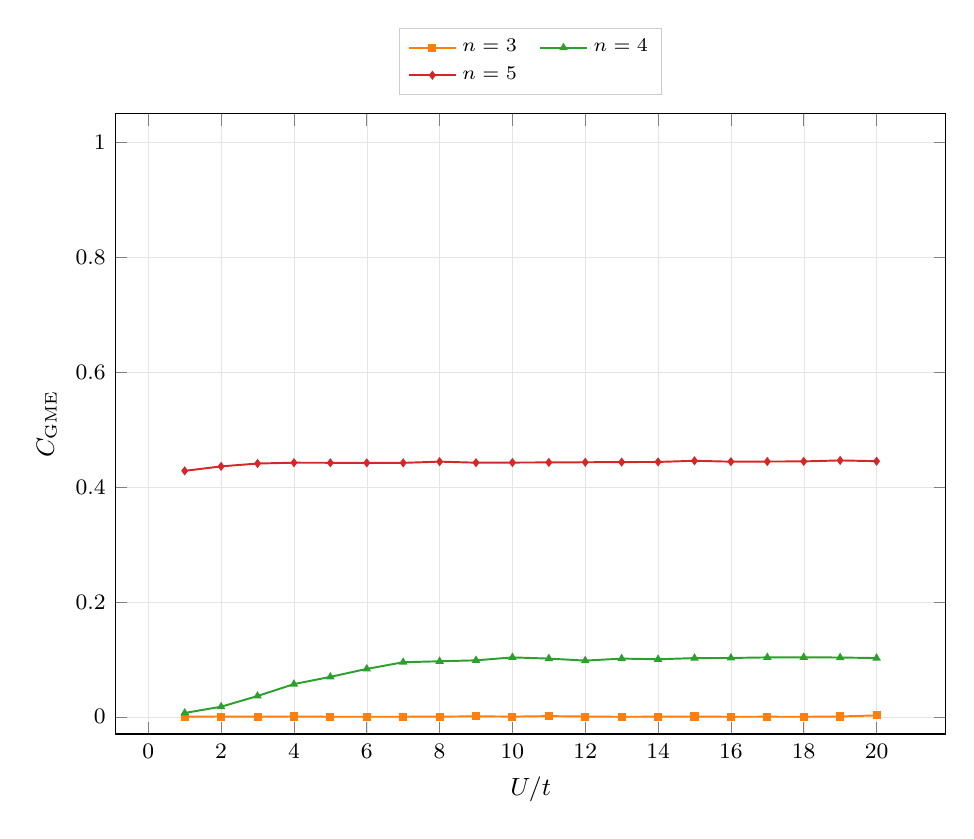
\begin{tikzpicture}
  \begin{axis}[
    width=\columnwidth,
    height=0.78\columnwidth,
    xlabel={$U/t$},
    ylabel={$C_{\mathrm{GME}}$},
    grid=both,
    grid style={line width=.1pt, draw=gray!20},
    tick label style={font=\footnotesize\rmfamily, /pgf/number format/fixed},
    label style={font=\small\rmfamily},
    scaled ticks=false,
    legend style={font=\scriptsize\rmfamily, draw=gray!40, at={(0.5,1.03)}, anchor=south, /tikz/every even column/.append style={column sep=6pt}},
    legend cell align={left},
    legend columns=2,
    ymin=-0.03,
    ymax=1.05,
  ]
    \addplot[color=gmeC1, mark=square*, mark size=1.1pt, line width=0.7pt] coordinates {
        (1,0.000363) (2,0.000511) (3,0.000167) (4,0.000551)
        (5,0.000058) (6,0.000123) (7,0.000136) (8,0.000254)
        (9,0.00088) (10,0.000314) (11,0.001216) (12,0.000476)
        (13,0.000015) (14,0.000271) (15,0.000519) (16,0.000021)
        (17,0.000204) (18,0.000033) (19,0.000554) (20,0.002451)
    };
    \addlegendentry{$n=3$}
    \addplot[color=gmeC2, mark=triangle*, mark size=1.1pt, line width=0.7pt] coordinates {
        (1,0.006699) (2,0.017545) (3,0.036225) (4,0.05694)
        (5,0.069574) (6,0.083411) (7,0.095037) (8,0.096688)
        (9,0.098336) (10,0.103452) (11,0.101393) (12,0.09785)
        (13,0.101364) (14,0.10019) (15,0.102244) (16,0.102487)
        (17,0.103429) (18,0.103692) (19,0.103233) (20,0.102323)
    };
    \addlegendentry{$n=4$}
    \addplot[color=gmeC3, mark=diamond*, mark size=1.1pt, line width=0.7pt] coordinates {
        (1,0.428306) (2,0.436109) (3,0.441064) (4,0.44251)
        (5,0.442348) (6,0.442225) (7,0.442221) (8,0.444356)
        (9,0.442515) (10,0.442751) (11,0.443012) (12,0.443283)
        (13,0.443555) (14,0.44382) (15,0.445821) (16,0.444317)
        (17,0.444547) (18,0.444764) (19,0.446481) (20,0.445159)
    };
    \addlegendentry{$n=5$}
  \end{axis}
\end{tikzpicture}
